Intro...

\section{Update Equations in parallel}

- consider calc of updated $U^{n+1}_i$, from $U^{n}_i$ for $\Omega_i$. 

- Introduce regular partitioning $\bar{\Omega} = \cup_{e} \bar{\Omega}_e$

- Introduce $\Gamma^{PEC}$ and $\Gamma^{ABC}$

- define internal faces $\Gamma^{I}$

- divide load by assign to $\Omega^p$ -  define partitioning of $\Omega^p$

- Parallelisation is achieved by assigning computation of the values $U^{n+1}_i$ from $U^{n}$ for each element $\Omega_e \in \Omega^p$ to a processor $P^p$.

- Define internal + external adjacent elements & internal, external and interface elements

% *****mention converse relationship internal/external ??

- Calculations on internal elements can happen easily...

Cals on external elements needs communication....say how

We communicate all the values

**** HOW DO WE MINIMISE COMMUNICATION
    -> partitioning
    -> sending all at once
**** HOW WE DO PREPROCESSING ON PARALLEL CODE
    -> how to establish lists of elements to send (need to do some comms here)
    -> establish lists of indexes in preprocessor
    -> contiguous buffers
    -> sendtoall (advantages of this)
    -> use processor numbering - and how does this work?
        ->
**** Identifying faces/elements in large meshes
**** HOW DO WE COMMUNICATE THESE VALUES
**** WHAT INDEXING DO WE NEED TO USE (i.e. how do we list these)
**** ANYTHING ELSE (?)

\subsubsection{Implementation detail}

Communication is an expensive operation with a significant overhead associated with each connection established [].
%[how much overhead? How expensive]. 
The number of messages can be reduced by collecting all the values of $U_{n}$ to be sent to any one 
destination processor and sending in a single message per time step.

Additionally should choose $\Omega^p$ such that we minimise both the number of messages and the number of values of $U_{n}$ to communicate.

% other processor has to know who they're from!! Talk about this in implementation
% [note: there could also a minimisation condition on the number of unknowns]
% note: there are a lot of factors at play here - first I want to minimise the number of communications established.....easy - i communicate once up front.
% - minimse the number of elements in $L^p$ (number of intersection of faces)
% - minimise the number of unknowns (weighting)
% - minimise the number of comms

This is equivalent to minimising the number of elements in $\cup_p L^p$ [more here!]. Deciding which elements should be contained in $\Omega^p$ is done using parMETIS [], a public-domain library which implements several algorithms for optimal partitioning of graphs.

The parMETIS library requires that each processor builds an element connectivity graph for a subset of all elements $\Omega_e$, where each element is uniquely referred to by a global numbering shared between all processors. The global numbering scheme established by the meshing software is used. The ranges of element numbers are divided equally amongst the processors by number ranges, not necessarily connected, and a graph built for subset of elements. Each node of the graph represents and element in the initial partition and each vertex represents a shared face or edge of two elements. 

The connectivity information is obtained by first constructing a node connectivity list, which for each node lists the elements which contain that node. This list is constructed by reading the whole mesh connectivity information and associating each read element which all the nodes it contains. The connectivites for all elements is read - however since these are integer values memory usage is not considered relevant [give an example of a very large mesh]. We loop through all faces of the elements allocated to this processor and for each face perform a loop on the nodes within that face. Within the inner loop we construct a list of connected elements [what is this]. The connected face will be the element in this list which appears the same number of times as the number of nodes in the face.

From the connectivity graph, parMETIS can then optimise the partitions in such a way to reduce the number of faces shared across processors. The resulting partition is shown for a circle with 5 processors in \figref{parmetis-figure}

The result of the optimisation by parMETIS is a list of all elements allocated to this processor and a number between 1 and the total number of processors (or equivalently the number of parts into which the domain is partitioned) which indicated the processor on which calculations should be performed (or equivalently the parition in which this element belongs). We allow each partition of the domain to correspond to a partitioning $\Omega^p$.

\section{Communication Arrays and Data Partition}

Recall that in order to implement the parallelised DG method it is not sufficient to distribute computations, some values of solution need to be communicated at each time step. In order to simplify the extension of a serial code to multiple processors the strategy employed involves establishing the set of elements that, for a given processor $A$, share a face with an element in the partition allocated to processor $A$. Nodal solution values for these elements are copied from the processor on which they are calculated to processor $A$ at each time step. The data partition is show in \figref{parmetis-figure} and results in a number local elements on which calculations are performed on this processor and a number of interface elements for which nodal solution values are available without calculation. By this data partition method code to calculate the numerical flux contributions does not need to distinguish betweeen local elements and interface elements.

** I need to talk here about how I set up the communication arrays, what else needs doing? what communication is required in pre-processing stage? etc **
** question: why do I need to keep track of the original numbering scheme? (i.e. localElementMap) **

\begin{figure}[htbp!]
 \centering
 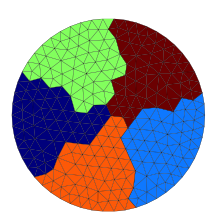
\includegraphics[width=0.3\textwidth]{Figures/Parallelisation/parmetisPartition}
 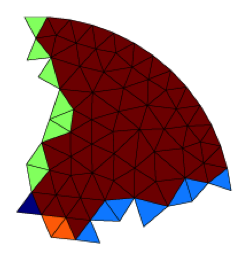
\includegraphics[width=0.2\textwidth]{Figures/Parallelisation/parmetisDataPartition}
\caption{Left: Partition of a circle given by parMETIS. Each color represents a different processor on which calculations for that processor should be performed. Right: Data partition of elements for a single processor (red) for circle}
\label{parmetis-figure}
\end{figure}

The nodal values to communicate between processors is be established in the preprocessing state, prior to computation. By parsing the graph and communication each processor recieves a list of elements for computation and the processors to which their nodal values should be sent and a list of interface elements ordered by processors number on which calculations occur. The vector of unknowns $U$, is implemented as a 1-dimensional array. By using the sendtoall functions available through the MPI library the elements numbering can be done in such a way that the MPI buffer recieved is a contiguous section of the vector U. this removes the need for a map of nodal values or copying values between the MPI buffer and the vector $U$.

The solution can be advanced in time following the exact procedure as the serial code, for a single partition of the domain per processor, provided that at each stage of the RK4 method the the nodal solution values should are communicated.

\section{Ordering of Faces}
